\section{SONU�LAR VE �NER�LER}
Sonu� olarak robotlar�n hayat�m�zdak� �nemi ve kolayl��� g�z �n�nde bulundurularak bir proje geli�tirilmi�tir. 
Yap�lan robotlar�n ilk amac� mesafe �l�en sens�rler sayesinde engllere �arpmadan ortamda gezinmesi ve uzaktan kumandayla kontrol edilmesidir. 

Bu projenin esnekli�i sayesinde ilerleyen a�amalarda ihtiya� duyulan entegre edilebilmesidir.

Robot resmini Sayfa 16'ya �ekil \ref{fig:arac_kul_2}'da g�sterilmi�tir. 

 \begin{figure}[h]
    \centering
    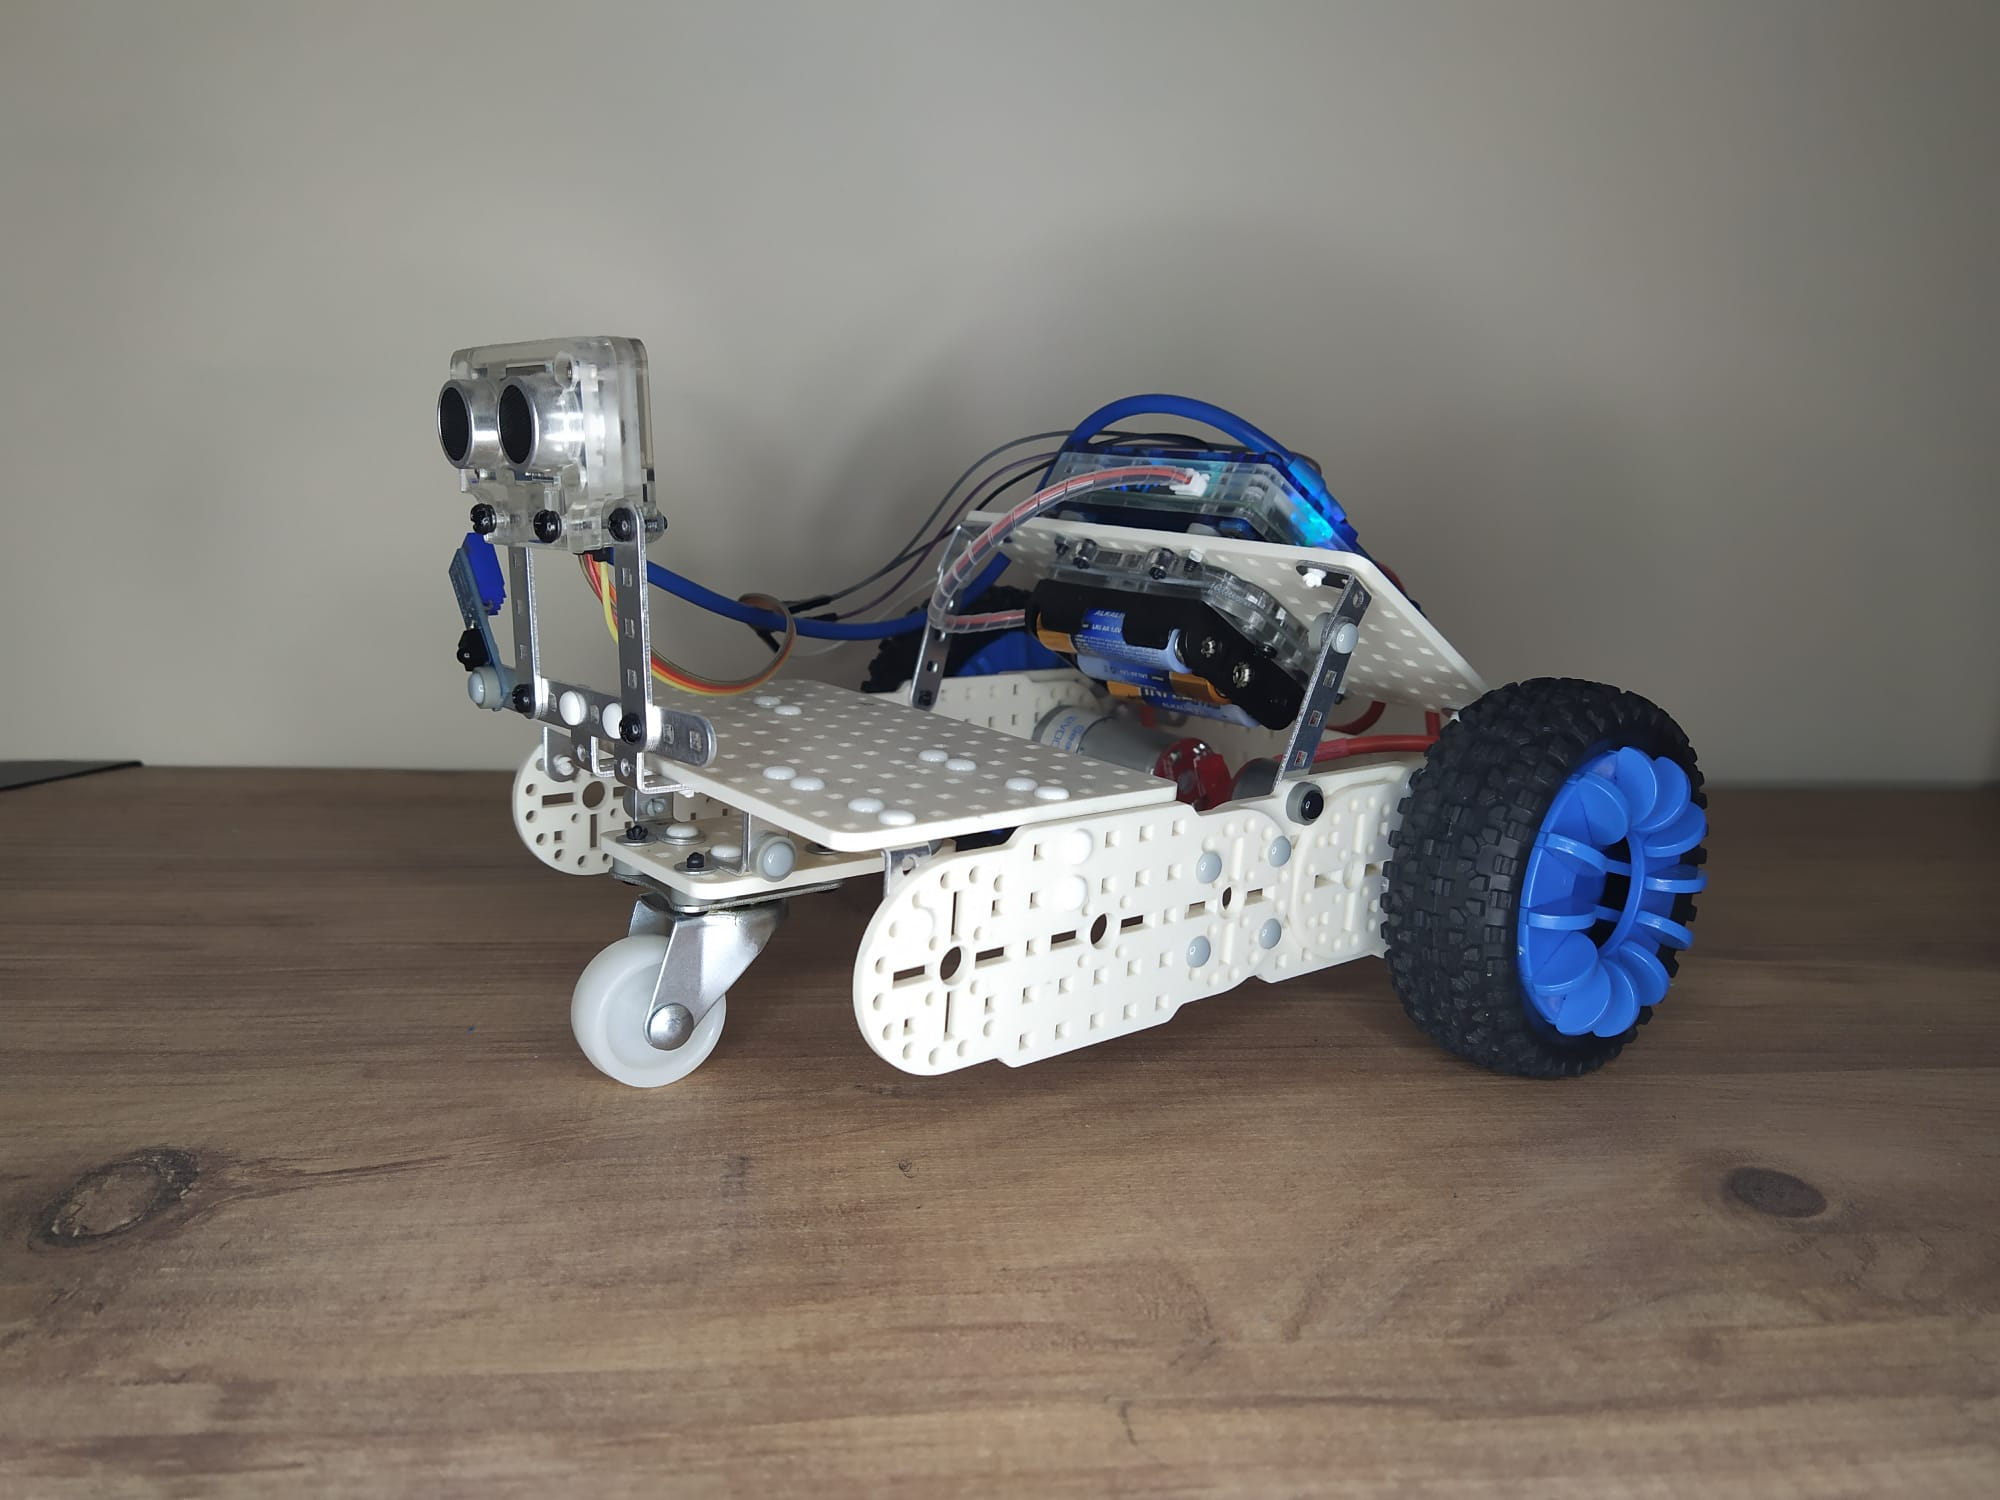
\includegraphics[scale=0.2]{arac_2}
    \caption{Projede kullan�lan Multiplo ara� kiti}
    \label{fig:arac_kul_2}
 \end{figure}


Bu projede ger�ekle�tirdi�imiz uygulamarlar video linkleri\\
Kumanda ile hareket ettirmek: \url{https://youtu.be/oysrP-Nnc1M}\\
Engel alg�lmak: \url{https://youtu.be/eq6jHHT1qb0}




 
